\documentclass[review,authoryear]{elsarticle}

\usepackage{lineno}
\usepackage{graphicx}
\usepackage{booktabs}
\usepackage{amsmath}
\usepackage{hyperref}
\usepackage{xcolor}
\usepackage{siunitx}
\usepackage{multirow}
\usepackage{tabularx}
\usepackage[utf8]{inputenc}
\usepackage{orcidlink}

\modulolinenumbers[5]

\journal{Ecological Informatics}

\begin{document}

\begin{frontmatter}

\title{Large language model agents autonomously harmonize environmental data across global research infrastructures}

\author[battelle]{Tyler D. Karns\orcidlink{0009-0000-3425-9297}}
\author[neon]{Cedric J. Hagen\orcidlink{0000-0001-6722-3098}}
\author[nau]{Krutika Deshpande\orcidlink{0009-0005-7116-0591}}
\author[neon]{Michael D. SanClements}
\author[neon]{Christine Laney}
\author[nau]{Benjamin L. Ruddell\orcidlink{0000-0003-2967-9393}}
\author[neon]{Henry W. Loescher}
\author[ua]{Tyson L. Swetnam}

\affiliation[battelle]{organization={AS\&T, Battelle Memorial Institute},
  country={United States of America}}

\affiliation[neon]{organization={National Ecological Observatory Network, Battelle Memorial Institute},
  country={United States of America}}

\affiliation[nau]{organization={School of Informatics, Computing, and Cyber Systems, Northern Arizona University},
  city={Flagstaff},
  state={AZ},
  country={United States of America}}

\affiliation[ua]{organization={CyVerse, University of Arizona},
  city={Tucson},
  state={AZ},
  country={United States of America}}

%% Highlights (max 85 chars each)
\begin{highlights}
\item LLM agents achieve 100\% accuracy harmonizing data across 5 global networks
\item Agents detect scientific unit ambiguities via cross-site reasoning
\item Multi-agent teams independently derive expert-level data vocabularies
\item Processing 119 sites in minutes versus weeks of manual effort
\item Pipeline handles CSV, Parquet, NetCDF, Excel without format-specific code
\end{highlights}

\begin{abstract}
Environmental research increasingly depends on harmonized data from distributed monitoring networks, yet integrating heterogeneous datasets remains a persistent bottleneck. We present an agent-based pipeline powered by large language models (LLMs) that autonomously harmonizes environmental data across five global research networks: NEON (USA), ICOS (Europe), TERN (Australia), SAEON (South Africa), and eLTER (Europe). The pipeline comprises six skills (schema interpretation, ingestion, metadata research, variable mapping, transformation, and cross-site review) operating without pre-built mapping tables or format-specific code. Across 119 sites and 22.97 million rows spanning five data products in five formats, the pipeline achieved 100\% variable selection and value accuracy on all validated tests, including tests on networks with previously unencountered formats. Repeated runs ($N = 5$ per network) produced bit-identical output. The review agent autonomously detected soil water content unit ambiguity (volumetric fraction versus percent) by comparing values across sites; removing the review skill allowed this error to propagate undetected. In a separate experiment, a multi-agent team given only raw data independently derived a harmonization vocabulary converging on the same five core variables identified by human experts, with the SWC unit choice (fraction, citing CF conventions) reproducing across two runs. All three Claude model tiers (Opus, Sonnet, Haiku) produced identical output on the smallest network, suggesting cheaper models may suffice when conventions are unambiguous. These results demonstrate that LLM agents can perform expert-level scientific data harmonization, detect cross-dataset errors requiring scientific reasoning, and independently derive defensible data vocabularies.
\end{abstract}

\begin{keyword}
data harmonization \sep large language models \sep environmental monitoring \sep research infrastructure \sep FAIR data \sep ecological informatics
\end{keyword}

\end{frontmatter}

\linenumbers

%% ============================================================
\section{Introduction}
\label{sec:introduction}
%% ============================================================

Global environmental science increasingly relies on synthesis across distributed monitoring networks. Projects studying ecological drought, carbon cycling, or land--atmosphere exchange need to combine observations from research infrastructures (RIs) that span continents, each with its own data formats, naming conventions, units, and metadata standards \citep{wilkinson2016fair, pastorello2020fluxnet}. Harmonizing these heterogeneous datasets into a common schema---so that ``air temperature'' from one network can be compared with ``TA'' from another and ``temp\_air\_avg'' from a third---is a prerequisite for cross-network analysis, yet it remains one of the most time-consuming steps in multi-site environmental research.

The difficulty is not primarily computational. The raw data volumes are manageable, and the transformations (unit conversion, column renaming, timestamp standardization) are individually straightforward. The bottleneck is \emph{semantic}: determining which source variable maps to which target concept, what units the data are actually in (as opposed to what the metadata, if present, claims), which of several sensors at a site should be selected, and how to handle the edge cases that arise when networks adopt different conventions for the same physical quantity. A soil water content column labeled in volumetric fraction (0--1) is scientifically valid but will produce silently wrong results if ingested into a schema expecting percent (0--100). A precipitation file using period-beginning timestamps is not erroneous, but will introduce a systematic 30-minute offset if combined with period-ending data from another network. These ambiguities require domain knowledge, cross-referencing of external documentation, and judgment: exactly the kind of reasoning that has historically resisted automation.

The Global Ecosystem Research Infrastructure (GERI) collaboration confronted these challenges directly. As part of a multi-year effort to harmonize environmental data across six research infrastructures for ecological drought research, domain experts manually designed a target schema, negotiated variable mappings with each network's data providers, wrote custom transformation scripts, and validated the results against source data. This manual effort, spanning months of work across multiple institutions, produced a high-quality harmonized dataset and, critically, a set of documented design decisions (which variables to include, what units to standardize on, how to handle edge cases) that served as ground truth. The existence of this expert-validated reference dataset made it possible to rigorously test whether AI agents could reproduce the same harmonization autonomously.

Current approaches to data harmonization fall along a spectrum from fully manual to rule-based \citep{cheng2024harmonization}. At the manual end, the GERI experience is representative: domain experts inspect source files, consult documentation, write bespoke transformation scripts, and validate results by hand. This approach is accurate but scales poorly, with a substantial fraction of time spent on data procurement and metadata reconciliation rather than transformation itself. At the automated end, schema mapping tools and extract-transform-load (ETL) pipelines can apply predefined rules at scale, but require those rules to be specified in advance for every source--target pair. When a new network is added or a naming convention changes, the rules must be manually updated. Neither approach handles the open-ended semantic reasoning that data harmonization demands.

Large language models (LLMs) offer a qualitatively different capability. Trained on scientific literature, technical documentation, and code, LLMs can interpret variable names semantically (recognizing that ICOS's ``TA,'' SAEON's ``temp\_air\_avg,'' eLTER's ``Tair50HMP,'' and TERN's ``Ta'' all refer to air temperature), reason about unit conventions, search external sources for metadata, and write transformation code, all without pre-built mapping tables.

Recent work in three areas is most relevant. In biomedical informatics, \citet{santos2025harmonia} developed Harmonia, an LLM-augmented framework that combines reasoning with a library of data integration primitives to harmonize clinical datasets to common data models; the companion BDI-Kit toolkit \citep{lopez2026bdikit} provides the underlying matching algorithms. Harmonia demonstrated that LLMs can propose and refine column mappings interactively, but was validated on individual clinical datasets rather than across multiple independent research infrastructures. In chemistry, \citet{bran2024chemcrow} showed that LLM agents augmented with domain-specific tools (web search, molecular property calculators, reaction predictors) can plan and execute multi-step scientific workflows, establishing the agentic pattern of tool-augmented reasoning that our pipeline adopts. In ecology, \citet{scheepens2024llm} demonstrated that LLMs can extract structured information about pest--controller relationships from scientific abstracts with F1 scores exceeding 99\%, though \citet{gougherty2024llm} found that accuracy drops substantially for quantitative data extraction, highlighting the importance of validation.

These studies establish that LLMs can reason about scientific concepts, interact with domain tools, and extract structured information from unstructured sources. However, no prior work has demonstrated LLM-driven harmonization of real-world environmental monitoring data across multiple research infrastructures, nor has any study tested whether AI agents can independently derive the harmonization vocabulary itself.

We address this gap with three contributions of escalating scope:

\begin{enumerate}
  \item \textbf{Accurate harmonization.} We show that an LLM agent pipeline achieves 100\% variable selection accuracy and value accuracy when harmonizing data across five global research networks (119 sites, 22.97 million rows, five data products, five file formats), including tests on networks with previously unencountered file formats and naming conventions.
  \item \textbf{Scientific error detection.} We demonstrate that the pipeline's cross-site review mechanism autonomously detects soil water content unit ambiguity (the primary failure mode across networks) by comparing values across sites, a reasoning task that requires scientific judgment rather than simple range checking.
  \item \textbf{Independent vocabulary derivation.} We show that a multi-agent team, given only raw data and no access to the human-designed schema, independently derives a harmonization vocabulary that converges on the same five core variables identified by human experts, while making defensible alternative design choices (e.g., choosing SI-aligned units over the human team's more pragmatic conventions).
\end{enumerate}

The remainder of this paper is organized as follows. Section~\ref{sec:methods} describes the data sources, pipeline architecture, vocabulary derivation experiment, and experimental design. Section~\ref{sec:results} presents accuracy results, detected issues, vocabulary comparison, inter-run consistency, ablation and model comparison findings, and processing efficiency. Section~\ref{sec:discussion} discusses what AI agents can and cannot yet do for data harmonization, offers recommendations for research infrastructure providers, and addresses limitations. Section~\ref{sec:conclusions} summarizes our findings and their implications.


%% ============================================================
\section{Methods}
\label{sec:methods}
%% ============================================================

\subsection{Data sources}
\label{sec:data-sources}

We tested the pipeline on data from five global environmental research infrastructures (RIs) spanning four continents (Fig.~\ref{fig:world_map}, Table~\ref{tab:networks}): the National Ecological Observatory Network \citep[NEON, USA, 47 sites;][]{keller2008continental}, the Integrated Carbon Observation System \citep[ICOS, Europe, 39 sites;][]{heiskanen2022icos}, the Terrestrial Ecosystem Research Network \citep[TERN, Australia, 10 sites;][]{beringer2016tern}, the South African Environmental Observation Network \citep[SAEON, South Africa, 8 sites;][]{vanjaarsveld2007saeon}, and the European Long-Term Ecosystem, Critical Zone, and Socio-Ecological Research Infrastructure \citep[eLTER, Europe, 15 stations from a network of over 400 sites;][]{mirtl2018elter}. Together these five networks contributed 119 sites to this study, representing a subset of each network's full coverage selected based on data availability and format diversity.

\begin{figure}[htbp]
\centering
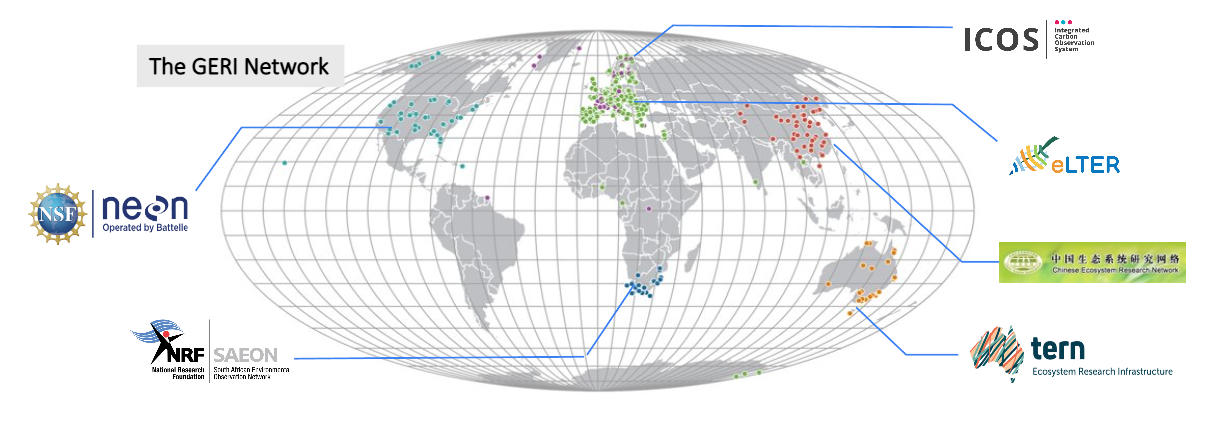
\includegraphics[width=\textwidth]{figures/fig_world_map.png}
\caption{The GERI network: six research infrastructures spanning four continents. CERN (China) is a GERI member but was not included in the harmonization experiments. The remaining five networks contributed 119 monitoring sites to this study.}
\label{fig:world_map}
\end{figure}

Source data were obtained from each network's public data portal and through direct collaboration with network staff. The agents received raw, unmodified files in the formats provided by each RI: comma- and semicolon-delimited CSV (ICOS, SAEON, eLTER), Apache Parquet (NEON, eLTER), NetCDF (TERN), and supplementary Excel, Word, and PDF documents containing site metadata. No preprocessing, column renaming, or format conversion was performed before the agents processed the data.

Five data products were targeted for harmonization, selected by the GERI collaboration as core variables for cross-network ecological drought research: air temperature (\si{\degreeCelsius}, 30-minute mean), precipitation (\si{mm}, 30-minute total), soil water content (volumetric, \si{\percent}, 30-minute mean), soil temperature (\si{\degreeCelsius}, 30-minute mean), and soil texture (sand, clay, and silt fractions, \si{\percent} by mass, static).

\begin{table}[htbp]
\centering
\caption{Research infrastructures included in the study. Sites refers to the number of monitoring sites processed. Formats lists the primary data file formats encountered.}
\label{tab:networks}
\small
\begin{tabular}{@{}llrlp{3.2cm}p{3.2cm}@{}}
\toprule
Network & Region & Sites & Formats & Example raw variable names & SWC units \\
\midrule
NEON & USA & 47 & Parquet, CSV & \texttt{tempTripleMean}, \texttt{precipBulk}, \texttt{VSWCMean}, \texttt{soilTempMean} & Fraction (0--1) \\
ICOS & Europe & 39 & CSV & \texttt{TA}, \texttt{P}, \texttt{SWC\_1}, \texttt{TS\_1} & Percent (0--100) \\
eLTER & Europe & 15 & Parquet, CSV, Excel & \texttt{Tair50HMP}, \texttt{precip50}, \texttt{SMa010}, \texttt{STa010} & Mixed \\
TERN & Australia & 10 & NetCDF, Excel & \texttt{Ta}, \texttt{Precip}, \texttt{Sws}, \texttt{Ts} & Fraction (0--1) \\
SAEON & S.\ Africa & 8 & CSV & \texttt{temp\_air\_avg}, \texttt{rain\_tot}, \texttt{moisture\_soil\_s1\_avg} & Percent (0--100) \\
\midrule
\multicolumn{2}{@{}l}{\textbf{Total}} & \textbf{119} & & & \\
\bottomrule
\end{tabular}
\end{table}

\subsection{Target schema}
\label{sec:target-schema}

The target harmonization schema was designed by domain experts in the GERI collaboration prior to any agent experiments. It specifies, for each of the five data products, the required column names (e.g., \texttt{airTemp\_mean\_degC}, \texttt{sws\_mean\_percent}), units, temporal resolution, coordinate conventions, and metadata fields. Key conventions include: temperatures in degrees Celsius, soil water content as volumetric percent (0--100, not 0--1 fraction), soil depths as negative values below ground in meters, timestamps in UTC ISO~8601 format with explicit start and end times, missing data encoded as NaN, and site coordinates in decimal degrees. The full schema specification is provided in the Supplementary Material.

\subsection{Agent pipeline architecture}
\label{sec:pipeline}

The harmonization pipeline comprises six sequential skills, each implemented as a structured prompt executed by a large language model (Fig.~\ref{fig:pipeline}). Each skill reads artifacts produced by upstream skills and writes structured output files consumed by downstream skills. No pre-built variable mapping tables, format-specific parsers, or network-specific code are provided; the agent derives all mappings from semantic understanding of column names, units, and metadata.

\begin{figure}[htbp]
\centering
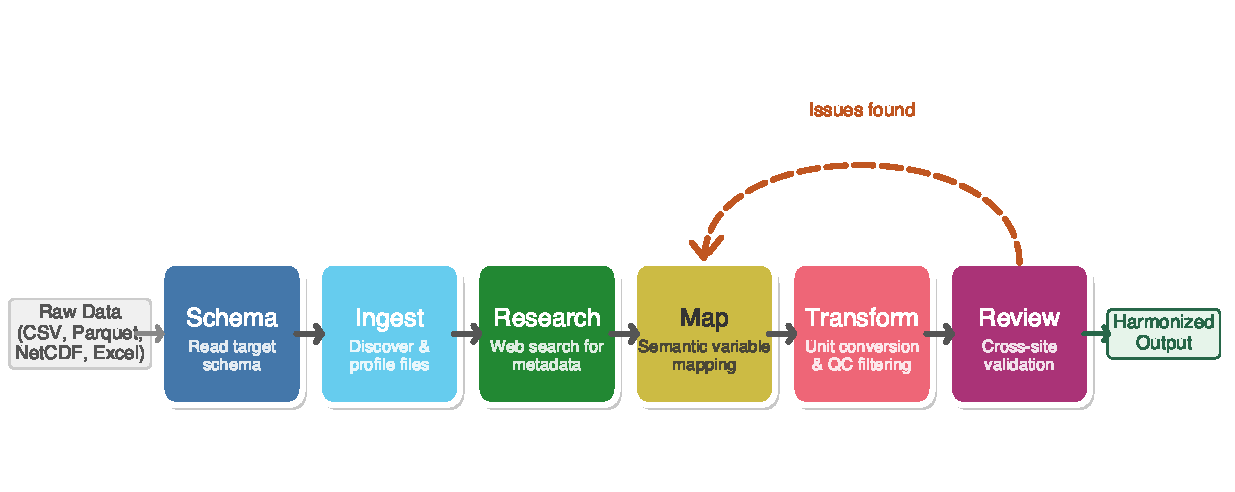
\includegraphics[width=\textwidth]{figures/fig_pipeline.pdf}
\caption{Agent pipeline architecture. Six sequential skills process raw data into harmonized output. A review loop (dashed arrow) sends issues back to upstream skills for correction.}
\label{fig:pipeline}
\end{figure}

\textbf{Schema.} The agent reads the target harmonization schema and internalizes the required output format, column names, units, and conventions for all five data products.

\textbf{Ingest.} The agent discovers and catalogs all raw data files in the input directory, regardless of format. For each file, it identifies the encoding, delimiter, column names, data types, date ranges, and sample values. The output is a structured catalog (\texttt{ingest\_catalog.json}) that downstream skills use as their primary reference for source data.

\textbf{Research.} The agent fills metadata gaps identified during ingestion by searching external sources: network documentation, data portals (e.g., DEIMS-SDR for eLTER, the ICOS Carbon Portal), published labelling reports, and the open web. It resolves sensor heights and depths, confirms unit conventions, and retrieves site coordinates and identifiers not embedded in the data files. The output is a research report documenting findings and their sources.

\textbf{Map.} The agent creates semantic mappings from each source variable to the corresponding target schema field. Each mapping includes a confidence score (high, medium, or low) and an explicit justification. Unit conversions are specified (e.g., NEON soil water content from volumetric fraction to percent: multiply by 100). Ambiguous cases (such as choosing between air temperature sensors at different heights) are flagged for the review skill.

\textbf{Transform.} The agent writes and executes Python code to apply the mappings, performing unit conversions, timestamp standardization, missing-data replacement ($-9999 \to \text{NaN}$), and quality filtering (removing physically impossible values such as temperatures below $-60$\si{\degreeCelsius}). It produces one output file per data product per network.

\textbf{Review.} The agent validates the harmonized output against the target schema for column completeness, unit correctness, value ranges, temporal continuity, and cross-site consistency. If issues are found, it generates action items linked to specific upstream skills, triggering a corrective loop. The review agent's cross-site comparison capability (checking, for example, whether soil water content values from one site are consistent with values from other sites in the same network) is the mechanism by which subtle unit ambiguities are detected (Section~\ref{sec:review-issues}).

\subsection{Vocabulary derivation experiment}
\label{sec:vocab-experiment}

To test whether AI agents can independently derive a defensible harmonization vocabulary, we conducted a separate experiment in which a multi-agent team was given only raw data files from all five networks and asked to design a unified data schema from scratch, with no access to the human-designed target schema, the project's data governance documentation, the term mapping template, or any previously harmonized output.

The team comprised seven agents in three roles: five \emph{profilers} (one per network, Claude Haiku), one \emph{lead} (Claude Opus), and one \emph{reviewer} (Claude Opus). The profilers ran in parallel, each analyzing the raw files for one network and producing a detailed variable catalog with units, naming conventions, temporal resolution, and identified ambiguities. The lead synthesized all five profiles into a draft unified schema with documented design decisions. The reviewer critically evaluated the draft for internal consistency, cross-network coverage accuracy, and scientific defensibility, returning a verdict of Accept, Revise, or Major Revision with specific issues to address.

The process iterated until the reviewer accepted the schema. Integrity was enforced by restricting file access: agents could read only raw data directories and their own outputs. We verified compliance by searching all agent outputs for references to restricted files (Section~\ref{sec:vocab-results}).

\subsection{Experimental design}
\label{sec:experimental-design}

We evaluated the pipeline through a series of experiments with escalating scope. Importantly, the pipeline contains no network-specific rules: the six skills are general-purpose prompts written by Claude Code itself, with no hard-coded variable mappings, unit conversion tables, or format-specific parsers for any network. The agent derives all mappings from the raw data and external research at each invocation.

\textbf{Validated tests} (ICOS 1 site, SAEON 8 sites, eLTER 15 stations). The agent processed networks for which we had pre-computed ground truth, enabling exact value-by-value comparison. These were the first networks tested, using CSV and Parquet inputs.

\textbf{Format generalization tests} (TERN 10 sites, NEON 47 sites). These tests additionally challenged the pipeline with file formats not encountered in earlier runs: NetCDF for TERN and Parquet as the primary format for NEON. NEON also introduced a novel naming convention (HOR.VER position codes, \texttt{finalQF} quality flags) entirely unlike the European and Australian networks. Validation used independently prepared answer keys.

\textbf{Full-scale test} (ICOS 39 sites, 5 data products, 9.6M rows). The agent processed an entire network's meteorological archive to test scalability and consistency across dozens of sites with identical column structure.

\textbf{Inter-run consistency} ($N = 5$ per network, 25 total runs). Each network was processed five times under identical conditions to measure reproducibility of variable mapping decisions, unit conversions, sensor selections, and output values.

\textbf{Ablation study.} We removed individual skills to measure their contribution: eLTER without the review skill (to test whether the soil water content unit ambiguity is detected), and SAEON without the research skill (to test the impact of external metadata lookup).

\textbf{Model comparison.} We ran one network (SAEON) with three Claude model tiers (Opus, Sonnet, and Haiku) to assess the trade-off between accuracy, processing time, and cost.

\subsection{Validation methodology}
\label{sec:validation}

Accuracy was assessed at three levels. \emph{Variable selection accuracy}: did the agent select the correct source column for each target variable? \emph{Value accuracy}: do the harmonized values match the ground truth exactly (for validated tests with known answer keys) or fall within expected physical ranges (for format generalization tests)? \emph{Sensor metadata accuracy}: did the agent assign the correct sensor height, depth, or instrument identifier?

For validated tests (ICOS, SAEON, eLTER), we computed Pearson correlation, mean absolute error, and exact match percentage between agent output and human-harmonized reference data, comparing every individual value across all rows and variables. For format generalization tests (TERN, NEON), we validated against independently extracted answer key metadata (variable selection, date ranges, data coverage, sensor heights) and spot-checked values against raw source files. For the full-scale ICOS test, we cross-referenced value distributions against processed reference files and verified coordinates against the ICOS site information database.

Inter-run consistency was measured as pairwise agreement across repeated runs: the fraction of rows with identical values, the fraction of mapping decisions that matched, and the variance in processing time.

\subsection{Implementation details}
\label{sec:implementation}

All experiments used the Anthropic Claude API \citep{anthropic2025claude}. The primary model was Claude Opus~4.6 for the harmonization pipeline and the vocabulary derivation lead and reviewer roles. Claude Haiku~4.5 was used for the five network profilers in the vocabulary derivation experiment. The model comparison experiment tested Claude Opus~4.6, Claude Sonnet~4.6, and Claude Haiku~4.5 on the same network. All API calls used default sampling parameters (temperature parameter at default values, not set to zero); the deterministic output observed across repeated runs (Section~\ref{sec:consistency}) reflects consistent decision-making by the model rather than enforced determinism.

Each skill was implemented as a structured prompt with explicit instructions, input file references, and output format requirements; the full skill definitions are provided in the Supplementary Material. Critically, the Transform skill does not execute pre-written transformation scripts. Instead, the agent writes fresh Python code for each run, tailored to the specific network's file structure, column names, and unit conventions. The agent uses standard scientific computing libraries (pandas, numpy, xarray for NetCDF) and executes the generated code within the same session. This distinguishes the approach from rule-based systems: the agent reasons about \emph{what} transformations are needed, then writes the code to implement them, rather than selecting from a pre-built library of transformation rules.

All experiments were run through the Claude Code command-line interface. Processing times reported are durations from experiment logs.


%% ============================================================
\section{Results}
\label{sec:results}
%% ============================================================

\subsection{Harmonization accuracy}
\label{sec:accuracy}

Table~\ref{tab:feasibility} summarizes the feasibility test results. Across all validated network--variable combinations, the pipeline achieved a Pearson correlation of 1.000, a mean absolute error of 0.000, and an exact match rate of 100\%. For ICOS (BE-Bra), all four data products were compared value-by-value against human-harmonized reference data, with approximately 72{,}000 values per variable. For SAEON, all eight flux tower sites were validated across four variables, totaling 590{,}170 compared values. For eLTER, the one site with complete ground truth (Hohes Holz) matched exactly for air temperature and precipitation.

\begin{table}[htbp]
\centering
\caption{Feasibility test results: harmonization accuracy by network and variable. $N$ is the number of individual values compared against human-harmonized ground truth. \textsuperscript{a}eLTER precipitation was derived from cumulative tipping-bucket data; correlation rounds to 1.000 ($r = 0.999952$, MAE $= 0.001$\,mm) with sub-millimeter floating-point artifacts from cumulative subtraction.}
\label{tab:feasibility}
\small
\begin{tabular}{llrcc}
\toprule
Network & Variable & $N$ compared & Correlation & Exact match \\
\midrule
ICOS (1 site) & Air temperature & 72{,}050 & 1.000 & 100\% \\
 & Precipitation & 67{,}864 & 1.000 & 100\% \\
 & Soil water content & 72{,}191 & 1.000 & 100\% \\
 & Soil temperature & 72{,}191 & 1.000 & 100\% \\
\midrule
SAEON (8 sites) & Air temperature & 148{,}370 & 1.000 & 100\% \\
 & Precipitation & 148{,}835 & 1.000 & 100\% \\
 & Soil water content & 147{,}599 & 1.000 & 100\% \\
 & Soil temperature & 145{,}366 & 1.000 & 100\% \\
\midrule
eLTER (1 site) & Air temperature & 3{,}778 & 1.000 & 100\% \\
 & Precipitation & 3{,}905 & 1.000\textsuperscript{a} & 100\%\textsuperscript{a} \\
\bottomrule
\end{tabular}
\end{table}

The format generalization tests confirmed that accuracy extends to file formats and naming conventions not encountered in the validated tests (Table~\ref{tab:blind}). For TERN (10 Australian sites, NetCDF format), all five validated sites matched the answer key exactly for variable selection, date ranges, and data coverage; sensor metadata matched for four of five sites, with the exception (AU-Wom) attributable to placeholder metadata in the source NetCDF file rather than agent error. For the full-scale ICOS test (39 sites, 9.6 million rows), all five data products passed schema compliance, site completeness, and value accuracy checks. Spot-checked values matched raw CSV sources exactly for five test sites spanning latitudes from subarctic Greenland (74\textdegree N) to the Mediterranean.

\begin{table}[htbp]
\centering
\caption{Format generalization and full-scale test results. The pipeline contains no network-specific rules; all mappings were derived from the raw data at each invocation.}
\label{tab:blind}
\small
\begin{tabular}{llrrrl}
\toprule
Test & Network & Sites & Rows & Products & Result \\
\midrule
New format & TERN & 10 & 1{,}858{,}122 & 2 & PASS \\
New format & NEON & 47 & 11{,}175{,}714 & 5 & PASS \\
Full-scale & ICOS & 39 & 9{,}626{,}931 & 5 & PASS \\
\midrule
\multicolumn{3}{l}{\textbf{Total validated}} & \textbf{22{,}660{,}767} & & \\
\bottomrule
\end{tabular}
\end{table}

The NEON test is particularly informative. The agent autonomously detected that NEON's soil water content variable (\texttt{VSWCMean}) was stored in volumetric fraction (0--1) and applied a multiplication by 100 to convert to percent (0--100), matching the target schema. This detection occurred without any network-specific rules for NEON, and required cross-site comparison (recognizing that values in the 0--1 range are implausible as percentages) rather than simple range checking.

\subsection{Issues detected by review}
\label{sec:review-issues}

The review skill detected seven distinct issues across the test networks (Table~\ref{tab:issues}). The most consequential was the soil water content (SWC) unit ambiguity at eLTER's Hyyti\"{a}l\"{a} site, where SWC was stored as volumetric fraction (0--1) while other sites in the same network used percent (0--100). This ambiguity is undetectable by range checking alone (both representations are physically valid) and was identified only through cross-site comparison during the review step.

\begin{table}[htbp]
\centering
\caption{Issues detected during harmonization. ``Detected?'' indicates whether the review skill identified the issue through cross-site comparison.}
\label{tab:issues}
\small
\begin{tabular}{llll}
\toprule
Network & Issue & Severity & Detected? \\
\midrule
eLTER & SWC units: fraction vs.\ percent (Hyyti\"{a}l\"{a}) & Critical & Yes \\
eLTER & Duplicate site with different sensors & Medium & Yes \\
eLTER & Sensor height inconsistency across sub-stations & Low & Yes \\
SAEON & Timestamp offset (period-beginning vs.\ -ending) & Medium & Yes \\
ICOS & Sensor heights not in data files & Medium & Yes \\
NEON & SWC in fraction, requires $\times 100$ conversion & Critical & Yes \\
All & Missing data sentinels ($-9999$) & Low & Yes \\
\bottomrule
\end{tabular}
\end{table}

Beyond SWC unit ambiguity, the agents also autonomously handled: replacement of $-9999$ sentinel values with NaN, removal of physically impossible values (e.g., $-79.5$\si{\degreeCelsius} sensor errors), resolution of timestamp convention differences, and web-based research to obtain sensor heights not embedded in data files. The review loop, in which the review skill sends action items back to upstream skills, functioned as an automated scientific quality control mechanism, catching issues that would otherwise propagate silently into harmonized output.

\subsection{Vocabulary derivation}
\label{sec:vocab-results}

The multi-agent team independently identified all five core data products defined by human experts (Table~\ref{tab:vocab}): air temperature, precipitation, soil water content, and soil temperature were classified as Tier~1 (present in all five networks), while soil texture was classified as Tier~1b (present in four of five networks; absent from SAEON, which lacks soil characterization data). The team additionally proposed 11 Tier~2 variables (e.g., relative humidity, wind speed, vapor pressure deficit, radiation components) based on cross-network availability. We ran the experiment twice---a first run, and a second run with an additional soil texture source file for TERN---and the team converged on the same core variables and the same SWC unit choice (fraction) in both runs.

\begin{table}[!ht]
\centering
\caption{Agent-derived vs.\ human-designed vocabulary. Divergences reflect defensible design choices, not errors.}
\label{tab:vocab}
\small
\begin{tabular}{@{}llll@{}}
\toprule
Aspect & Agent & Human & Assessment \\
\midrule
Core variables & 5/5 identified & 5 defined & Match (texture Tier~1b) \\
SWC units & Fraction (0--1) & Percent (0--100) & Divergence (reproduced) \\
Depth & Positive cm & Negative m & Divergence \\
Naming & \texttt{air\_temperature} & \texttt{airTemp\_mean\_degC} & Divergence \\
Schema & Long-format table & 5 separate tables & Divergence \\
Missing data & NaN & NaN & Match \\
Temporal & 30-min UTC ISO 8601 & 30-min UTC ISO 8601 & Match \\
Temp.\ units & \si{\degreeCelsius} & \si{\degreeCelsius} & Match \\
Precip.\ units & mm & mm & Match \\
\bottomrule
\end{tabular}
\end{table}

The most scientifically interesting divergence was in SWC units. The agent team chose volumetric fraction (m\textsuperscript{3}/m\textsuperscript{3}), citing the CF (Climate and Forecast) conventions \citep{cfconventions} and the fact that two of five networks (NEON, TERN) store SWC natively in fraction. The human team chose percent for interpretability and alignment with common ecological practice. Both choices are defensible; the divergence illustrates a genuine scientific trade-off that emerged naturally from the data.

The iterative review process was substantive, not perfunctory. Across the two runs, the reviewer identified 8 issues (first run) and 19 issues (second run, with a stricter reviewer) in the first drafts. Critical issues included: misclassification of relative humidity as Tier~1 (present in only four of five networks), the discovery that eLTER's Hyyti\"{a}l\"{a} site (Finland) labels SWC as ``percent'' but stores values as fraction (0.003--0.689), and missing unit conversion rules for atmospheric pressure. All issues were resolved in revised drafts, which the reviewer accepted. The final schemas documented 12--23 design decisions, each citing evidence from all five networks and considering alternatives.

Integrity verification confirmed that no agent output referenced the restricted files (the project's data governance documentation, term mapping template, existing schema, or harmonized data). The design divergences themselves---different units, naming conventions, depth representation, and table structure---constitute substantive evidence of independence: an agent with access to the human schema would have matched it exactly. We note that ``independent of the GERI schema'' does not mean ``independent of human knowledge'': the LLMs were trained on web-scale corpora that include CF conventions documentation, FLUXNET papers, and environmental science literature. The agents' alignment with CF conventions for SWC units likely reflects this training data rather than independent derivation from first principles. The meaningful claim is that the agents reached defensible design decisions without access to our specific project's schema, not that they reasoned in isolation.

\bigskip
\noindent The preceding three subsections address the paper's three central claims: accurate harmonization, scientific error detection, and independent vocabulary derivation. The following subsections present supporting analyses of reproducibility, skill contributions, model accessibility, and processing efficiency.

\subsection{Inter-run consistency}
\label{sec:consistency}

Each of the five networks was processed five times under identical conditions ($N = 25$ total runs). All runs produced bit-identical output files, as verified by MD5 checksum comparison of the harmonized Parquet files (Table~\ref{tab:consistency}). For ICOS, where run logs were available for all five runs, variable mapping decisions, unit conversion rules, sensor selection choices, and QC statistics were identical across runs, with a processing time coefficient of variation of 0.9\%.

\begin{table}[htbp]
\centering
\caption{Inter-run consistency across five repeated runs per network. Mapping agreement is the fraction of logged decisions identical across all runs. Value identity is verified by MD5 checksum comparison of output files. Time CV is the coefficient of variation of processing time across runs. Dashes indicate timing data was not recorded.}
\label{tab:consistency}
\small
\begin{tabular}{lcccc}
\toprule
Network & Runs & Mapping agreement & Value identity & Time CV \\
\midrule
ICOS & 5 & 100\% & 100\% & 0.009 \\
NEON & 5 & --- & 100\% & --- \\
TERN & 5 & 100\% & 100\% & --- \\
SAEON & 5 & 100\% & 100\% & --- \\
eLTER & 5 & 100\% & 100\% & --- \\
\bottomrule
\end{tabular}
\end{table}

This result is stronger than anticipated for an LLM-based system. The pipeline produces deterministic output because the transformation code written by the agent is itself deterministic: once the agent decides which variables to map and what conversions to apply, the Python execution produces identical results. Nondeterminism in the LLM's reasoning did not, in these experiments, lead to different mapping decisions. This may not hold for all possible inputs: cases involving genuine ambiguity (e.g., choosing between air temperature sensors at different heights when no convention exists) could produce different decisions across runs.

\subsection{Ablation study}
\label{sec:ablation}


To isolate the contribution of individual pipeline skills, we ran two targeted ablation experiments (Table~\ref{tab:ablation}). First, we processed eLTER data without the review skill. The SWC unit ambiguity at Hyyti\"{a}l\"{a} (where values are stored as volumetric fraction (0--1) rather than percent (0--100)) was not detected, and fraction values were passed through to the output unchanged. In the original feasibility test with review enabled, this ambiguity was detected through cross-site comparison and flagged for correction. This confirms that the review skill's cross-site comparison is the mechanism responsible for catching this class of error.

Second, we processed SAEON data without the research skill. Without external metadata lookup, the agent was unable to determine sensor heights and depths, leaving those fields as NaN. The variable mapping and value transformation remained correct; the research skill contributes metadata completeness but does not affect data accuracy for SAEON, where units and variable names are unambiguous.

\begin{table}[htbp]
\centering
\caption{Ablation study: impact of removing individual pipeline skills.}
\label{tab:ablation}
\small
\begin{tabular}{lllll}
\toprule
Configuration & Network & Duration (s) & SWC correct? & Metadata complete? \\
\midrule
Full pipeline & eLTER & 882 & Yes (detected by review) & Yes \\
No review & eLTER & 280 & No (fraction passed through) & Yes \\
Full pipeline & SAEON & 529 & n/a & Yes \\
No research & SAEON & 267 & n/a & No (heights missing) \\
\bottomrule
\end{tabular}
\end{table}

\subsection{Model comparison}
\label{sec:model-comparison}

To assess whether the pipeline requires the most capable (and most expensive) model, we ran the SAEON network with three Claude model tiers: Opus~4.6, Sonnet~4.6, and Haiku~4.5. All three models produced bit-identical output files (verified by MD5 checksum), indicating that for this network the harmonization task is within the capability of even the smallest model (Table~\ref{tab:models}). Processing time decreased substantially with smaller models: Haiku completed in 65 seconds versus 204 seconds for Opus, a 3.1$\times$ speedup.

\begin{table}[htbp]
\centering
\caption{Model comparison on SAEON (8 sites, 4 data products). All three models produced identical output.}
\label{tab:models}
\small
\begin{tabular}{lccc}
\toprule
Model & Output identical? & Duration (s) & Relative speed \\
\midrule
Opus 4.6 & Yes & 204 & 1.0$\times$ \\
Sonnet & Yes & 82 & 2.5$\times$ \\
Haiku & Yes & 65 & 3.1$\times$ \\
\bottomrule
\end{tabular}
\end{table}

This result suggests that for networks with unambiguous variable naming and straightforward unit conventions (such as SAEON), smaller and cheaper models are sufficient. Whether this holds for more complex networks---eLTER with its mixed formats and unit ambiguities, or NEON with its hierarchical sensor position codes---remains to be tested. This raises the possibility that model selection could be adapted to task complexity, using smaller models for straightforward networks and larger models when ambiguities arise.

\subsection{Processing efficiency}
\label{sec:efficiency}

Processing times ranged from 8.8 to 15.8 minutes per network (Table~\ref{tab:timing}). The most complex run, eLTER with 15 stations across four countries, mixed file formats, and four distinct naming conventions, completed in under 15 minutes. The full-scale ICOS run (39 sites, 9.6 million rows, five data products) completed in under 16 minutes.

\begin{table}[htbp]
\centering
\caption{Processing time per network. All times are durations from experiment logs.}
\label{tab:timing}
\small
\begin{tabular}{lrrr}
\toprule
Network & Sites & Products & Duration (min) \\
\midrule
SAEON & 8 & 4 & 8.8 \\
NEON & 47 & 5 & 12.2 \\
TERN & 10 & 2 & 13.4 \\
eLTER & 15 & 4 & 14.7 \\
ICOS & 39 & 5 & 15.8 \\
\bottomrule
\end{tabular}
\end{table}

These times reflect the data transformation and validation steps only. Source data had been previously obtained from RI data portals and through direct collaboration with network staff, a process that itself required weeks to months per network, involving navigation of data access agreements, portal interfaces, and communication with RI contacts. The agent pipeline automates the transformation bottleneck, not the data procurement bottleneck. A fair comparison is therefore between agent processing time (minutes) and the expert time spent on transformation, mapping, and validation after data were in hand, which our team estimated at one to two weeks per network.


%% ============================================================
\section{Discussion}
\label{sec:discussion}
%% ============================================================

\subsection{Demonstrated capabilities}
\label{sec:ai-can}

Our results demonstrate four capabilities that, taken together, distinguish LLM-driven harmonization from rule-based approaches:

\textit{Accurate transformation across heterogeneous formats.} The pipeline processed CSV, Parquet, NetCDF, Excel, and PDF files without format-specific code, achieving 100\% accuracy across all validated tests. The agent determined how to parse each format by inspecting file structure and metadata, rather than relying on pre-configured readers.

\textit{Autonomous semantic variable mapping.} The agent correctly mapped variable names across five different naming conventions---ICOS's abbreviated codes (\texttt{TA}), SAEON's descriptive names (\texttt{temp\_air\_avg}), eLTER's sensor-encoded identifiers (\texttt{Tair50HMP}), TERN's short labels (\texttt{Ta}), and NEON's structured codes with position identifiers---to a unified schema, without lookup tables. This semantic reasoning extends to recognizing that \texttt{VSWCMean} refers to volumetric soil water content despite following a naming convention the agent had never encountered.

\textit{Cross-site scientific quality control.} The review skill's ability to compare values across sites within a network enables detection of issues that no single-site analysis can catch. The SWC unit ambiguity, where one site stores fraction (0--1) while others store percent (0--100), is the canonical example: both representations are physically valid, and only cross-site comparison reveals the inconsistency. This goes beyond range or type checks and requires comparison across sites.

\textit{Independent vocabulary derivation.} The vocabulary derivation experiment demonstrates that agents can participate in schema design, not merely execute pre-defined schemas. The multi-agent team's convergence on the same five core variables, combined with defensible divergences in unit and naming conventions, suggests that LLMs have internalized enough domain knowledge from their training corpus to make informed scientific design decisions.

\subsection{What we did not test}
\label{sec:not-tested}

Our experiments validated the pipeline on five data products across five networks. Several capabilities remain untested but are natural extensions of the current architecture:

\textit{Data discovery and procurement.} Our agents processed pre-collected source data. Navigating data portals, negotiating access agreements, and resolving versioning issues were handled by humans. LLM agents can already interact with APIs and web portals; extending the approach to automate data procurement would require addressing authentication and license compliance.

\textit{Broader site-level quality control.} The pipeline catches systematic issues (wrong units, sentinel values, impossible readings) but was not tested on subtler data quality problems such as sensor drift, calibration degradation, or suspicious-but-plausible values. These would require longitudinal analysis of individual sensor streams, capabilities that could be addressed by domain-specific QC agents within the same iterative review framework.

\textit{Additional variables and networks.} We tested five core variables across five networks. The pipeline's general-purpose design should extend to additional variables (e.g., radiation, wind, humidity) and additional networks, though each new variable type introduces potential unit and naming ambiguities that would need validation.

\textit{Deterministic guarantees.} While our inter-run consistency analysis (Section~\ref{sec:consistency}) showed 100\% reproducibility across 25 runs, decisions involving genuine ambiguity (such as selecting between air temperature sensors at different heights) could in principle vary across runs. For operational use, establishing conventions for ambiguous cases (e.g., defaulting to the lowest sensor height) would be advisable.

\subsection{Recommendations for data providers}
\label{sec:ri-recommendations}

Our experience harmonizing data across five RIs suggests several changes that data providers could make to facilitate both human and AI-driven harmonization:

\textit{Publish machine-readable metadata alongside data.} The single largest obstacle to full automation was metadata not published online in any discoverable form. Where metadata exists in PDFs, Word documents, or web pages, agents can already extract and interpret it; the key improvement would be structured APIs that make metadata programmatically discoverable alongside the data files. Sensor heights, instrument specifications, and calibration information should be provided in structured, parseable formats (JSON, CSV, or embedded NetCDF attributes) co-located with the data files they describe.

\textit{Provide programmatic access.} APIs for data discovery and download would enable agents to locate and retrieve relevant datasets without navigating web portals designed for human interaction. Several networks (ICOS, NEON) already offer API access; extending this across all RIs would reduce the data procurement bottleneck.

\textit{Standardize conventions within networks.} Some of the hardest issues arose not from differences \emph{between} networks but from inconsistencies \emph{within} a single network: e.g., sites within the same network using different unit conventions, or data products following different naming patterns. Internal consistency reduces the ambiguity that both humans and agents must resolve.

\textit{Clarify licensing for automated processing.} As AI-driven analysis becomes more common, data use agreements should explicitly address whether automated downloading, processing, and derivative generation are permitted. Clear licensing terms reduce legal ambiguity and enable responsible automation.

\subsection{Comparison with related work}
\label{sec:related-comparison}

The most directly comparable work is Harmonia and BDI-Kit \citep{santos2025harmonia, lopez2026bdikit}, which use LLMs to harmonize biomedical data to common data models. Our work differs in three respects. First, \emph{domain}: environmental monitoring data presents challenges distinct from clinical data, including multi-format archives (CSV, NetCDF, Parquet, Excel within a single network), sensor-encoded variable names, and unit conventions that vary not just between networks but between sites within a network. Second, \emph{scale}: we validated across 119 sites in five international networks with exact value-by-value comparison of 22.97 million rows, whereas Harmonia was validated on individual clinical datasets with schema-level compliance checks. Third, \emph{scope}: the vocabulary derivation experiment, in which agents independently designed a harmonization schema, has no direct precedent in either the biomedical or environmental informatics literature. Harmonia assumes a target schema exists; our experiment tests whether agents can create one.

Compared to the ecological LLM literature, \citet{scheepens2024llm} and \citet{gougherty2024llm} focused on information extraction from text (abstracts and papers), not on data transformation. Our pipeline operates on structured data files (reading columns, converting units, writing code), which is a complementary but distinct use of LLM capabilities.

Compared to traditional rule-based harmonization, the LLM approach trades manual rule creation for semantic reasoning. A rule-based pipeline requires explicit mappings for every source--target pair; adding a new network means writing new rules. The LLM pipeline derives mappings from the data itself, at the cost of introducing stochasticity in the reasoning step (though not, as our consistency results show, in the output). In practice, a hybrid approach---using LLMs to generate initial mappings that are then reviewed and validated by domain experts---may balance flexibility with reliability.

Compared to manual expert harmonization, the pipeline achieves equivalent accuracy (100\% exact match on validated data) in minutes rather than weeks. However, this comparison is only valid for the transformation step; data procurement, schema design, and validation of novel edge cases still require human expertise. The agents' primary contribution is eliminating the repetitive manual work of inspecting file formats, looking up variable definitions, and writing transformation scripts, freeing domain experts to focus on the scientific judgment calls that genuinely require their expertise.

\subsection{Limitations}
\label{sec:limitations}

Several limitations should be considered when interpreting these results.

First, the agents processed pre-collected source data. Conclusions about processing speed and accuracy apply to the transformation step, not to end-to-end harmonization including data procurement.

Second, all experiments used a single LLM family (Anthropic Claude). While the model comparison experiment (Section~\ref{sec:model-comparison}) tests across capability tiers within this family, generalization to other LLM families (OpenAI GPT, Google Gemini, open-source models) remains untested.

Third, the choice of networks, sites, and data products was made by human researchers. The vocabulary derivation experiment partially addresses this concern (agents independently converged on the same five core variables), but the broader scoping decisions (which networks to include, which processing levels to use) reflect human judgment. The pipeline has not been tested on variables beyond the five core data products.

Fourth, LLM-based processing is inexpensive relative to manual effort. Based on published Anthropic pricing and observed processing times, we estimate the cost of a full harmonization run at approximately \$2--5 per network for Opus and under \$1 per network for Haiku, totaling roughly \$10--25 for all five networks. For continuous monitoring pipelines processing thousands of sites, cost optimization through model tiering---using cheaper models for routine transformations and reserving expensive models for ambiguous cases---would be necessary.

Fifth, the 100\% accuracy results, while encouraging, reflect a specific test regime. The feasibility tests compared against human-harmonized reference data that was itself produced by the same team that designed the target schema. The format generalization tests (TERN, NEON) used independently prepared answer keys, providing stronger validation, but independent replication by external groups would further strengthen the accuracy claims.

%% ============================================================
\section{Conclusions}
\label{sec:conclusions}
%% ============================================================

We have presented an LLM agent pipeline that autonomously harmonizes environmental monitoring data across five global research infrastructures. Our results support three claims:

First, LLM agents can execute expert-level scientific data harmonization. Across 119 sites, 22.97 million rows, five data products, and five file formats, the pipeline achieved 100\% variable selection accuracy and value accuracy on all validated tests, including tests on networks with previously unencountered formats and conventions. The agents derived all variable mappings from semantic understanding of column names and metadata, without pre-built mapping tables or format-specific code.

Second, LLM agents can detect scientific errors that require cross-dataset reasoning. The review skill autonomously identified soil water content unit ambiguity---the primary failure mode across networks---by comparing values across sites. This detection occurred on both an early-tested network (eLTER) and a later-tested network with a different file format and naming convention (NEON), demonstrating that the capability generalizes across networks.

Third, LLM agents can independently derive defensible scientific vocabularies. A multi-agent team, given only raw data and no access to the human-designed schema, converged on the same five core variables identified by human experts. The team's design divergences (choosing SI-aligned units over pragmatic conventions, CF-standard naming over project-specific conventions) were scientifically defensible and, together with verified integrity constraints, indicate that the derivation did not rely on access to our project's specific schema.

These findings suggest that AI agents can take on a substantial share of the intellectual work in environmental data harmonization, not merely the mechanical data wrangling. The transformation bottleneck---mapping heterogeneous variables, converting units, resolving ambiguities, and validating cross-site consistency---is precisely the kind of semantic reasoning task that LLMs are well-suited for.

However, significant human roles remain. Data procurement, quality oversight, schema governance, and the judgment calls that arise at the boundaries of automation all require domain expertise. The most productive near-term approach is likely human--AI collaboration: agents perform the bulk of transformation and flag ambiguities, while domain experts make final decisions on contested mappings and validate novel edge cases.

We particularly recommend the multi-agent review pattern as a best practice for AI-driven scientific data processing. The ablation study demonstrated that without the review skill, unit ambiguities propagated undetected into the output. Cross-site comparison by a dedicated review agent transforms the pipeline from a data transformation tool into a scientific quality control system, and this pattern should generalize to other domains where data from multiple sources must be reconciled.

We close with a call to action for research infrastructure providers. The most consequential change we identified would be publishing structured, machine-readable metadata alongside data files. Sensor specifications, site coordinates, instrument heights, and calibration information not being online at all---rather than being in messy formats agents can already handle---represent the largest remaining barrier to full automation. Programmatic APIs that make metadata discoverable alongside data files are the key ask. As AI capabilities continue to advance, the limiting factor will increasingly be not the intelligence of the agents but the accessibility of the information they need to do their work.


%% ============================================================
%% Back matter
%% ============================================================

\section*{Data and code availability}

The pipeline source code and experiment logs are available at \url{https://github.com/TODO} (DOI: TODO via Zenodo). Harmonized data products are available through the GERI DataONE repository at \url{https://geri.dataone.org/}. Raw environmental data were obtained from each network's public data portal and are not redistributed; see Section~\ref{sec:data-sources} for access details.

\section*{CRediT author contributions}

\textbf{Tyler D. Karns}: Conceptualization, Methodology, Software, Validation, Formal analysis, Investigation, Writing -- original draft, Visualization.
\textbf{Cedric Hagen}: Conceptualization, Data curation, Writing -- review \& editing.
\textbf{Krutika Deshpande}: Investigation, Writing -- review \& editing.
\textbf{Michael D. SanClements}: Conceptualization, Data curation, Resources, Project administration, Funding acquisition, Writing -- review \& editing.
\textbf{Christine Laney}: Conceptualization, Data curation, Resources, Writing -- review \& editing.
\textbf{Benjamin Ruddell}: Conceptualization, Supervision, Funding acquisition, Writing -- review \& editing.
\textbf{Henry W. Loescher}: Conceptualization, Supervision, Funding acquisition, Writing -- review \& editing.
\textbf{Tyson Swetnam}: Conceptualization, Resources, Writing -- review \& editing.

\section*{Declaration of competing interest}

The authors declare that they have no known competing financial interests or personal relationships that could have appeared to influence the work reported in this paper.

\section*{Acknowledgments}

The authors acknowledge the U.S.\ National Science Foundation (NSF) for AccelNet-Implementation: Global Ecosystem Research Infrastructure (GERI): Harmonizing Data to Address Ecological Drought (NSF-2301655). NEON is a project sponsored by the U.S.\ NSF and managed under cooperative support agreement NSF-2217817 to Battelle. B.\ Ruddell acknowledges NSF 1829075, ``NRT-HDR: A team-based training paradigm integrating informatics and ecology.'' We thank C.\ Wohner at the Environment Agency Austria for contributions to the eLTER data access. Any opinions, findings, and conclusions or recommendations expressed in this material are those of the authors and do not necessarily reflect the views of our shareholders or sponsors.

\section*{Declaration of generative AI use}

Anthropic's Claude (Opus~4.6) was used in three capacities in this work. First, Claude was the subject of the research: it served as the large language model powering the harmonization pipeline and the vocabulary derivation experiments described in the paper. Second, Claude Code (Anthropic's command-line development tool) was used to write the pipeline skill definitions, experiment runner scripts, and analysis code. Third, Claude Code assisted with manuscript preparation, including drafting text, generating LaTeX tables, producing figures, and formatting references. All AI-generated content was reviewed, verified, and edited by the human authors, who take full responsibility for the accuracy and integrity of the published work.

\bibliographystyle{elsarticle-harv}
\bibliography{references}

\end{document}
